\subsection{SOUSLIN SPACES}

DEFINITION 2. A topological space X is said to be a Souslin space if it is metrizable and if there exists a Polish space P and a continuous mapping of P onto X. A subset A of a topological space X is called a Souslin set if the subspace A is a Souslin space.

Clearly every Polish space is Souslin, and the image of a Souslin space X under a continuous mapping of X into a metrizable space Y is a Souslin space.

PROPOSITION 4. Every Souslin space X is of countable type.

Let P be a Polish space and f a continuous mapping of P onto X. Then the image under f of a countable dense subset of P is a countable dense subset of X.

PROPOSITION 5. Every closed (resp. open) subspace of a Souslin space X is Souslin.

For if \(f\) is a continuous mapping of a Polish space \(\mathbf{P}\) onto \(\mathbf{X}\) , then the inverse image under \(f\) of a closed (resp. open) subset of \(\mathbf{X}\) is a closed (resp. open) subset of \(\mathbf{P}\) , hence is a Polish subspace of \(\mathbf{P}\) (no. 1, Propositions 1 and 2).

PROPOSITION 6. Let X be a Souslin space, let Y be a Hausdorff space and let \(f: \mathbf{X} \to \mathbf{Y}\) be a continuous mapping. Then the inverse image under \(f\) of a Souslin subspace A of Y is a Souslin subspace of \(\mathbf{X}\) .

Let P, Q be Polish spaces, let g be a continuous mapping of P onto X and let h be a continuous mapping of Q onto A. Let R be the set of all \((x,y)\in\mathbf{P}\times\mathbf{Q}\) such that \(f(g(x))=h(y)\) ; R is closed in \(P\times Q\) and is therefore a Polish subspace of \(P\times Q\) (no. 1, Proposition 1). Let \(\varphi\) be the restriction to R of the projection \(pr_{1}\) . Then the subspace \(\overline{f}^{1}(\mathbf{A})\) of X is the image of R under the continuous mapping \(g\circ\varphi\) and is therefore a Souslin space.

PROPOSITION 7. The product and the sum of a countable family of Souslin spaces are Souslin spaces.

For each integer n, let \(X_{n}\) be a metrizable space, \(P_{n}\) a Polish space, and \(f_{n}\) a continuous mapping of \(P_{n}\) onto \(X_{n}\) . The product (resp. sum) of the spaces \(P_{n}\) is Polish (no. 1, Proposition 1), and the image of this space under the mapping which is the product of the \(f_{n}\) (resp. the mapping which agrees with \(f_{n}\) on \(P_{n}\) for all n) is the product (resp. sum) of the spaces \(X_{n}\) ; the latter is metrizable, and is therefore a Souslin space.

PROPOSITION 8. Let X be a metrizable space and let \((\mathbf{A}_{n})\) be a sequence of Souslin subspaces of X. Then the union and the intersection of the \(A_{n}\) are Souslin spaces.

These subspaces are certainly metrizable. The existence of the canonical map of the sum of the \(A_{n}\) onto the subspace \(\bigcup A_{n}\) of X shows that the latter is a Souslin space; and \(\bigcap_{n} A_{n}\) is Souslin by virtue of Propositions 5 and 7 and Lemma 1 of no. 1.

\pandocbounded{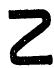
\includegraphics[keepaspectratio]{images/part002_bec1605a.jpg}}

In general, even in a Polish space, the complement of a Souslin subspace is not necessarily Souslin (cf.~Exercise 6); see, however, no. 6, Theorem 2, Corollary.

PROPOSITION 9. Let X be a metrizable space, and let A be a relatively compact Souslin subspace of X. Then there exists a compact metrizable space K, a decreasing sequence \((\mathbf{B}_{n})\) of subsets of K, each of which is a countable union of compact sets, and a continuous mapping \(f: K \to X\) , such that \(A = f\left(\bigcap_{n} B_{n}\right)\) .

Replacing X by \(\overline{\mathbf{A}}\) if necessary, we may suppose that X is compact and that A is dense in X. Since A is a Souslin space, there is a Polish space P and a continuous mapping \(g: \mathrm{P} \to \mathrm{X}\) such that \(g(\mathrm{P}) = \mathrm{A}\) . By no. 1, Theorem 1, Corollary 1, we may assume that P is the intersection of a decreasing sequence \((\mathbf{U}_n)\) of open subsets of the cube \(\mathbf{I}^{\mathbf{N}}\) . Let K be the space \(\mathbf{I}^{\mathbf{N}} \times \mathbf{X}\) , which is compact and metrizable (§ 2, no. 4, Theorem 1, Corollary 2). Let \(\mathbf{G} \subset \mathbf{P} \times \mathbf{X}\) be the graph of \(g\) , let \(\overline{\mathbf{G}}\) be the closure of G in K, and let \(f\) denote the projection of \(\mathbf{K} = \mathbf{I}^{\mathbf{N}} \times \mathbf{X}\) onto X; then clearly we have \(f(\mathbf{G}) = \mathbf{A}\) . Since \(g\) is continuous, G is closed in \(\mathbf{P} \times \mathbf{X}\) (Chapter I, § 8, no. 1, Proposition 2, Corollary 2) and \(\mathbf{G} = \overline{\mathbf{G}} \cap (\mathbf{P} \times \mathbf{X})\) ; hence \(\mathbf{G} = \bigcap_{n=1}^{n} \mathbf{B}_n\) , where

\[
\mathbf {B} _ {n} = \overline {{\mathbf {G}}} \cap (\mathbf {U} _ {n} \times \mathbf {X}).
\]

Since each \(U_{n}\) is a countable union of closed sets in \(I^{N}\) (§ 2, no. 5, Proposition 7), each \(B_{n}\) is a countable union of compact sets and the proof is complete.

